\chapter{不確定性、エーレンフェストの定理、古典極限}

\section{線形ハミルトニアンに残された課題}

この模型
\begin{equation}
H=cP
\label{eq:l10-linear-hamiltonian}
\end{equation}
は、その波動束が形を変えずに平行移動するため有用であった。しかし、重大な警告も伴っている。運動量は正にも負にもなり得るので、同じ式が一方の平面波には正のエネルギーを、他方には負のエネルギーを割り当てる：
\begin{equation}
\psi_p(x)=e^{ipx/\hbar},
\qquad
E(p)=cp.
\end{equation}
もし任意に多くの物理的粒子が負エネルギーの状態を占めることができれば、真空は最低エネルギーの状態ではなくなる。真空は正のエネルギーの量子を生成し、その補償として新たな粒子に負のエネルギーを預けることができ、全エネルギーを保ちながら真空を際限なく下げてしまう。

\begin{classroomqa}
\audiencequestion{負エネルギーの枝は、単にエネルギーの零点を奇妙に選んだというだけのことではないのはなぜか。}
\lecturerresponse{すべてのエネルギーに共通の定数を加えることは無害である。非有界なスペクトルはそれとは異なる。もし正のエネルギーの粒子が釣り合いを持ち去る一方で、より低いエネルギーの状態がいくらでも占有され得るならば、安定な基底状態は存在しない。安定性のためには、真空に対する下限が必要である。}
\end{classroomqa}

\begin{figure}[htbp]
\centering
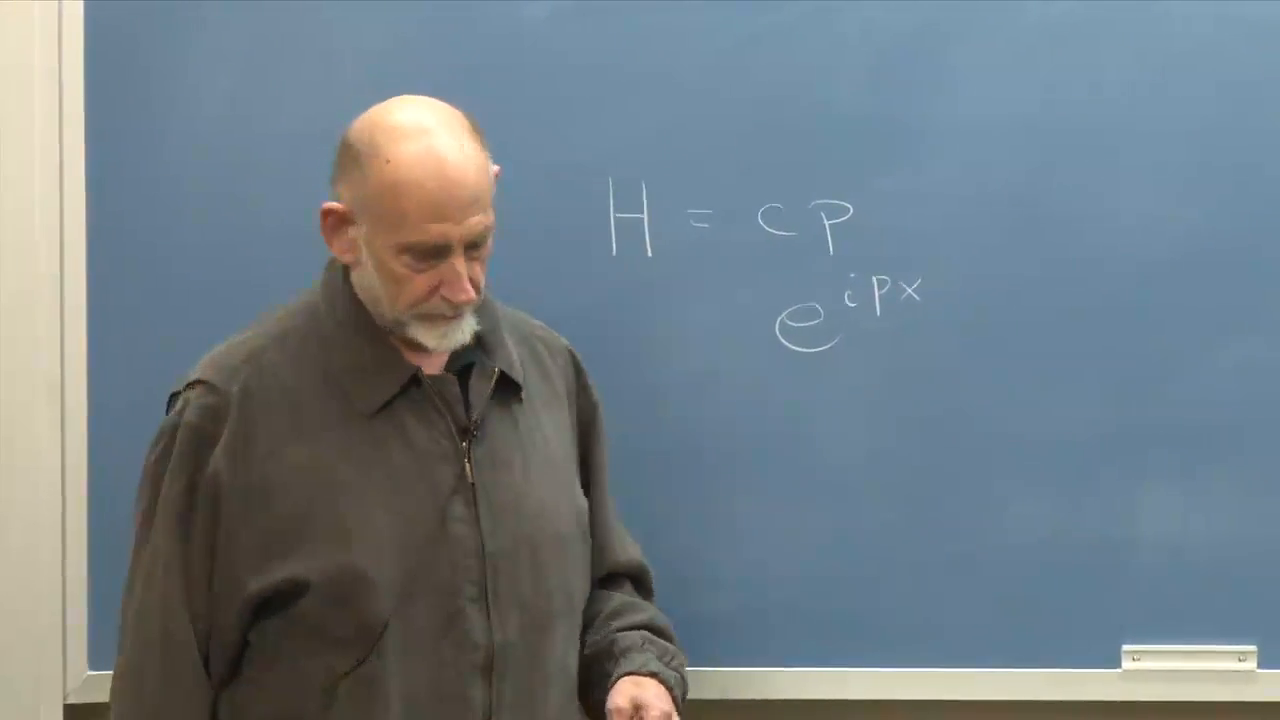
\includegraphics[width=0.88\textwidth]{lecture_10_figure_01.png}
\caption{線形ハミルトニアンとその平面波固有関数は、\(p<0\)のとき負エネルギーの枝を露わにする。}
\lectureframe{00:04:35}
\end{figure}

ディラックの歴史的な答えはフェルミオンに対して有効であった。フェルミオンは排他原理に従う。すなわち、二つの同一なフェルミオンが同じ一粒子状態を占めることはできない。すべての負エネルギーの状態を埋め尽くすと想像しよう。それらがすべて占められると、排他原理によって別のフェルミオンがその領域へ落ち込むことが妨げられる。埋め尽くされた集合の中の空孔は反粒子として振る舞う。

この議論は負エネルギーのボソンを救わない。任意の数のボソンが一つの状態を占めることができるので、負エネルギーのボソン的モードは際限なく占有され得る。古い「満たされた海」の描像は、反粒子への歴史的な道筋として見るのが最も適切である。現代の量子場の理論は、物理的真空を観測可能な負エネルギー電子の文字通りの海として扱うことなく、粒子と反粒子を組織化する。ここで必要な論点はより狭い。すなわち、この玩具的ハミルトニアンは完全で安定な粒子の理論ではないということである。

固定された速さで運動するフェルミオン的粒子の一次元の戯画として、この模型はディラックの考えが関連していたニュートリノ問題をほのめかす。しかし光子の理論として用いることはできない。光子はボソンであり、排他原理はその負エネルギーの状態を埋めて遮断することができないからである。

\begin{classroomqa}
\audiencequestion{なぜ排他原理はフェルミオン的構成を安定化できるが、ボソン的構成はできないのか。}
\lecturerresponse{フェルミオン的状態は一度占められると遮断される。ボソン的状態にはそのような占有の上限がないので、負エネルギーのボソン的モードは依然としてエネルギーを際限なく下げることを許してしまう。}
\end{classroomqa}

\paragraph{ここで講義が現在立っている位置。}
この四半期では、量子力学の基礎の多くと、いくつかの意図的に単純な系を展開してきたが、応用はごくわずかである。特に、調和振動子にさえまだ到達していない。この省略は終わりではなく境界を示している。次に相対性理論と場の理論が来て、その後、振動子およびその上に築かれた他の構造を研究するために量子力学を再び取り上げなければならない。以前のエンタングルメントの議論に対する持続的な関心もまた、基礎的な道筋が価値あったことを示している。

この見通しのもとで、残された課題は閉じられる。主たる課題は波動関数、不確定性、そして量子論的発展と古典力学の関係である。目的は可能な限り最も一般的な発展方程式ではなく、もともとSchr\"odingerによって書かれた特別な位置空間の方程式である。

\section{波動関数と完全可換座標}

直線上の一粒子に対して、位置空間の波動関数は
\begin{equation}
\psi(x)=\braket{x}{\psi},
\end{equation}
であり、粒子を\(x\)の近くに見出す確率振幅である。運動量空間の波動関数は
\begin{equation}
\widetilde{\psi}(p)=\braket{p}{\psi}.
\end{equation}
である。これらは同じ抽象的状態を異なる基底で記述し、フーリエ変換によって関係づけられる：
\begin{align}
\psi(x)
&=
\int_{-\infty}^{\infty}
\frac{dp}{\sqrt{2\pi\hbar}}\,
\widetilde{\psi}(p)e^{ipx/\hbar},
\label{eq:l10-fourier-forward}\\
\widetilde{\psi}(p)
&=
\int_{-\infty}^{\infty}
\frac{dx}{\sqrt{2\pi\hbar}}\,
\psi(x)e^{-ipx/\hbar}.
\label{eq:l10-fourier-inverse}
\end{align}

\begin{figure}[htbp]
\centering
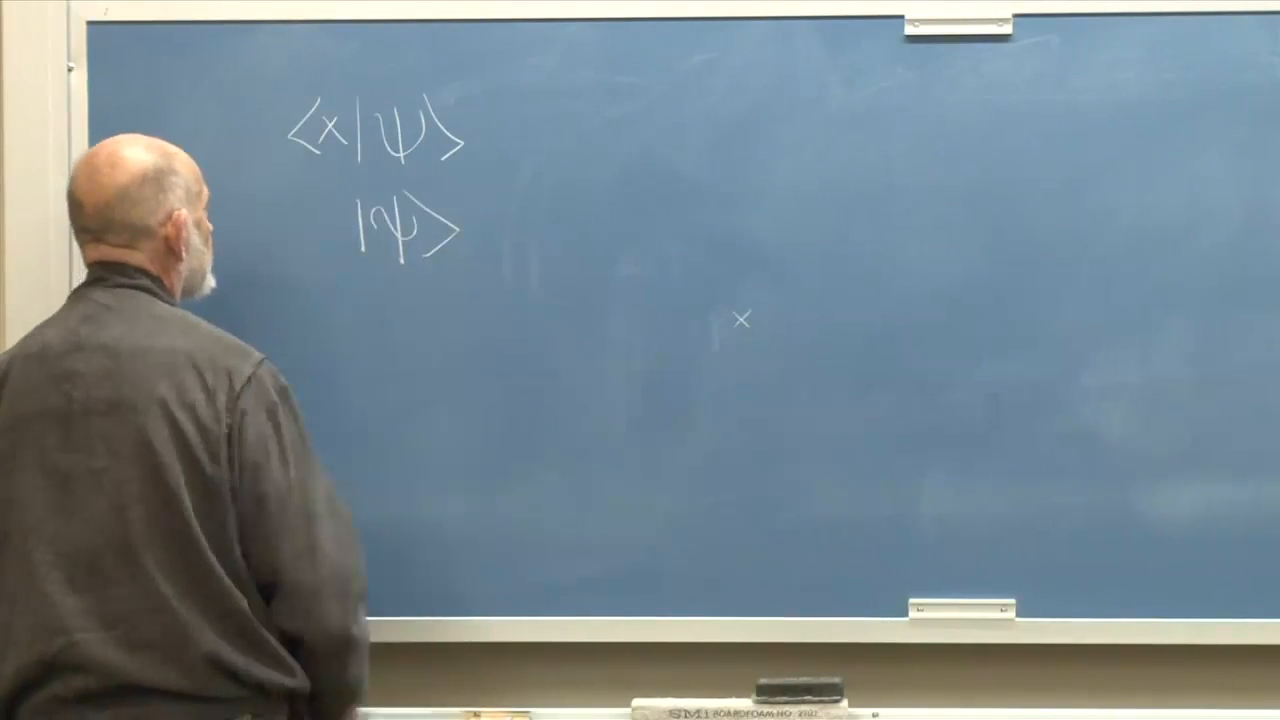
\includegraphics[width=0.88\textwidth]{lecture_10_figure_02.png}
\caption{位置と運動量の波動関数は、一つの状態を二つの異なる連続基底へ射影したものである。}
\lectureframe{00:09:05}
\end{figure}

二次元空間では、\(X\)と\(Y\)は可換であるため、共通の固有基底を両方の座標でラベル付けでき、波動関数は\(\psi(x,y)\)となる。この可換性は抽象的な公理だけから強制されるものではなく、通常の空間に対する経験的に成功した量子論的記述の一部である。三次元の\(N\)粒子に対して、
\begin{equation}
\psi(\mathbf{x}_1,\ldots,\mathbf{x}_N)
\end{equation}
は配位空間上の関数であり、各粒子に独立に付随する別々の三次元波動ではない。したがって、巨視的な系は膨大な数の座標を必要とし得る。

\begin{classroomqa}
\audiencequestion{異なる空間座標の可換性は量子力学から自動的に従うのか。}
\lecturerresponse{否。抽象的枠組みは多くの可観測量の代数を許容する。異なるデカルト位置成分が可換であるという事実は、通常の空間における粒子の量子力学に関する経験的な構造的事実である。}
\end{classroomqa}

すべての座標をフーリエ変換してすべての運動量の波動関数を得ることも、選択した変数のみを変換することもできる。混合表示は正当である。なぜなら表示は基底の選択であり、物理的状態の変化ではないからである。

\section{不確定性が測るもの}

不確定性原理の最も原始的な形はフーリエ対から直ちに従う。確定した運動量の状態は一定の絶対値をもつ平面波であり、位置の局在をもたない。位置に鋭く局在した状態は多くの運動量成分を必要とする。より一般には、フーリエ対の一方を狭めると他方が広がる。

\begin{figure}[htbp]
\centering
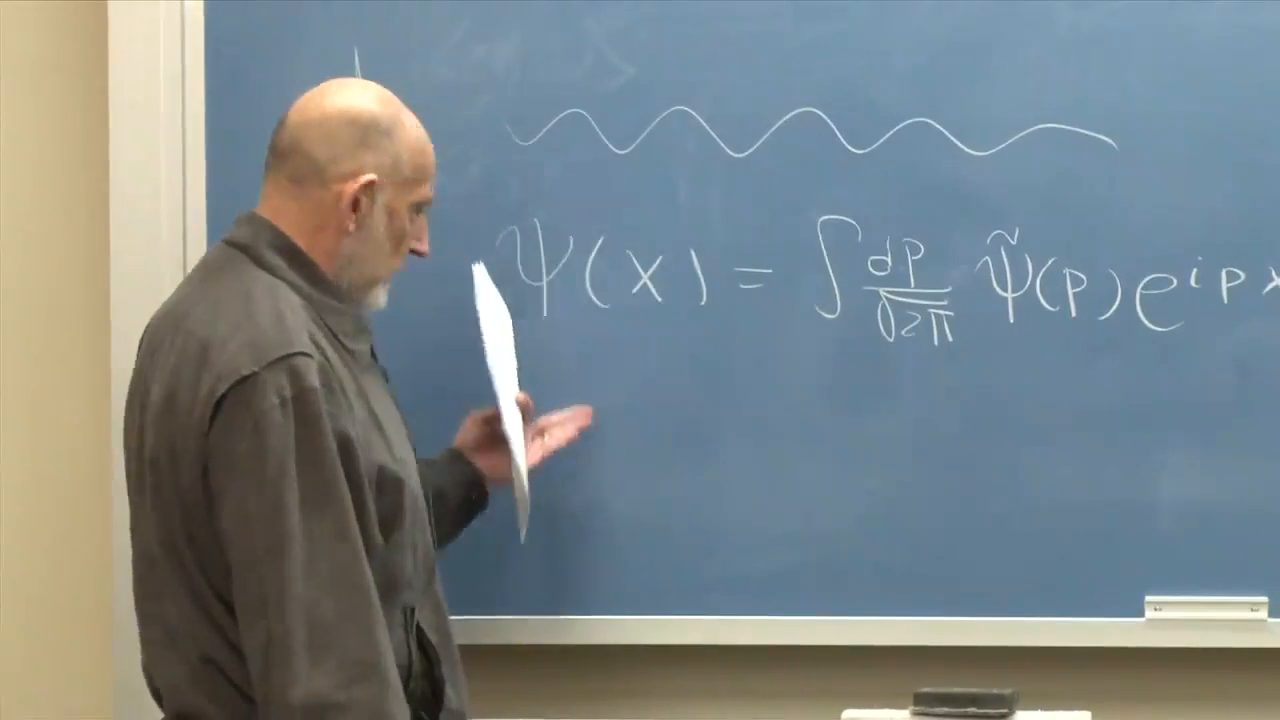
\includegraphics[width=0.88\textwidth]{lecture_10_figure_03.png}
\caption{局在した位置プロファイルは、逆運動量表示における平面波の広い重ね合わせを必要とする。}
\lectureframe{00:14:45}
\end{figure}

この記述を定量的にするには、一般の可観測量\(Q\)から始める。正規化された状態におけるその期待値は
\begin{equation}
\expect{Q}=\bra{\psi}Q\ket{\psi}.
\end{equation}
分散は
\begin{equation}
(\Delta Q)^2
=
\expect{\bigl(Q-\expect{Q}\bigr)^2}
=
\expect{Q^2}-\expect{Q}^2.
\label{eq:l10-general-variance}
\end{equation}
不確定性\(\Delta Q\)はこの分散の正の平方根である。

位置については、まず原点を移動して\(\expect{X}=0\)とできる。すると
\begin{equation}
(\Delta x)^2
=
\expect{X^2}
=
\int_{-\infty}^{\infty}
dx\,|\psi(x)|^2x^2.
\label{eq:l10-position-variance}
\end{equation}
正と負の寄与は\(\expect{X}\)では相殺するが、\(\expect{X^2}\)では加算される。したがって、より広い確率分布はより大きな分散をもつ。

\begin{figure}[htbp]
\centering
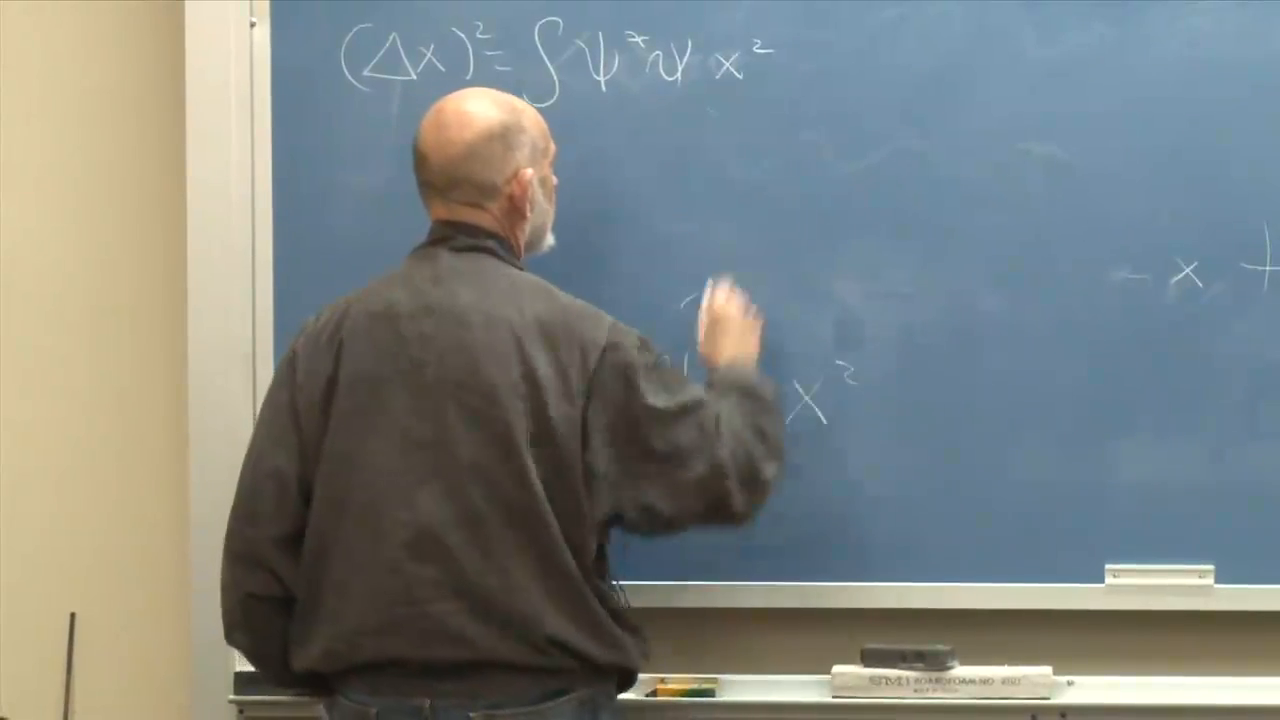
\includegraphics[width=0.88\textwidth]{lecture_10_figure_04.png}
\caption{平均をゼロに移動すると、位置の分散は\(x^2\)の確率重み付き積分である。}
\lectureframe{00:20:50}
\end{figure}

\(\expect{X^2}\)と\(\expect{X}^2\)の区別は本質的である。ゼロに関して対称な分布は\(\expect{X}=0\)をもつが、原点に集中していない限り依然として\(\expect{X^2}>0\)をもつ。

運動量の分散は運動量空間で直接定義できる：
\begin{equation}
(\Delta p)^2
=
\int_{-\infty}^{\infty}
dp\,|\widetilde{\psi}(p)|^2
\bigl(p-\expect{P}\bigr)^2.
\end{equation}
証明には位置空間で作業する方がより有用である。平均運動量をゼロに移動し、
\begin{equation}
P=-i\hbar\frac{d}{dx},
\qquad
P^2=-\hbar^2\frac{d^2}{dx^2}.
\end{equation}
を用いると
\begin{equation}
(\Delta p)^2
=
\expect{P^2}
=
-\hbar^2
\int_{-\infty}^{\infty}
dx\,\psi^*(x)\frac{d^2\psi}{dx^2}.
\label{eq:l10-momentum-variance-second}
\end{equation}

\begin{classroomqa}
\audiencequestion{位置空間の式が負号で始まるとき、分散がどのように正になり得るのか。}
\lecturerresponse{その負号に掛かる積分は非正である。部分積分により一つの微分が\(\psi^*\)に移り、二つ目の負号が導入され、結果は絶対値の二乗の積分に変わる。}
\end{classroomqa}

無限遠で十分速く減衰する波動関数に対して、
\begin{equation}
\int f\,g'\,dx
=
\left[fg\right]_{-\infty}^{\infty}
-
\int f'g\,dx,
\end{equation}
であり、境界項は消える。これを式~\eqref{eq:l10-momentum-variance-second}に一度適用すると
\begin{equation}
(\Delta p)^2
=
\hbar^2
\int_{-\infty}^{\infty}
dx\,
\frac{d\psi^*}{dx}
\frac{d\psi}{dx}
=
\hbar^2
\int_{-\infty}^{\infty}
dx\,
\left|\frac{d\psi}{dx}\right|^2
\geq 0.
\label{eq:l10-momentum-variance-positive}
\end{equation}

\begin{figure}[htbp]
\centering
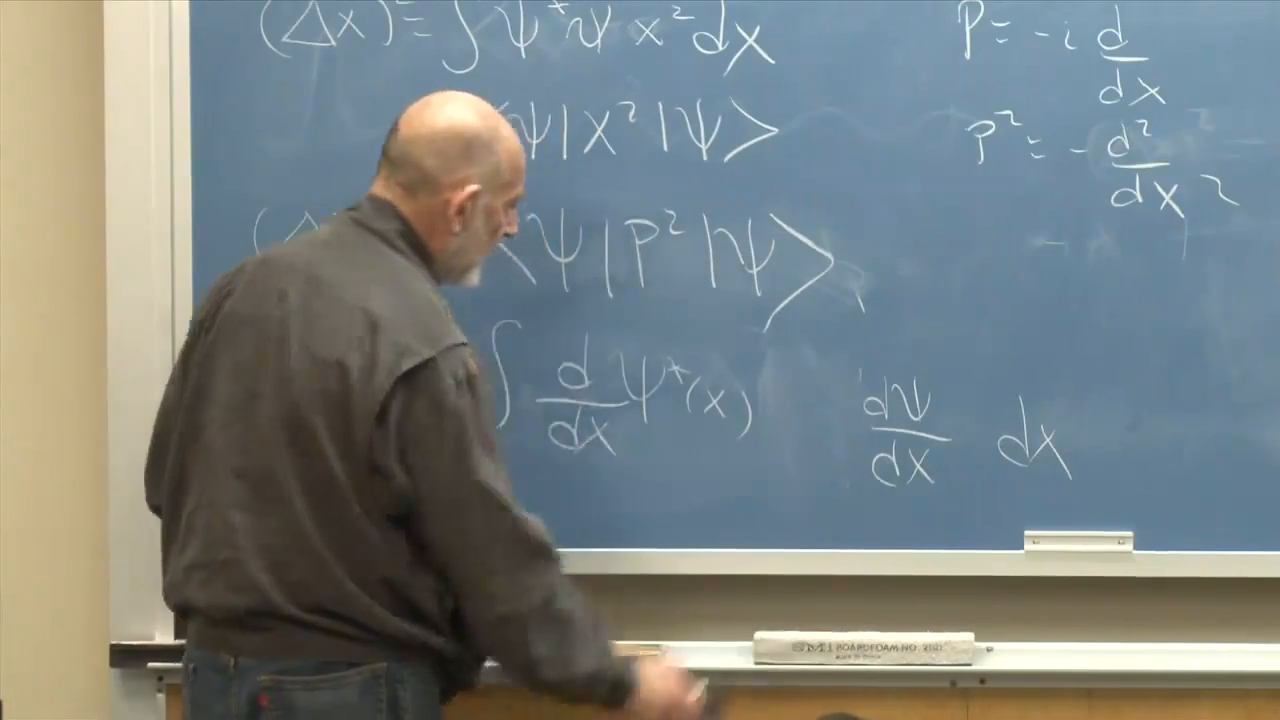
\includegraphics[width=0.88\textwidth]{lecture_10_figure_05.png}
\caption{部分積分により、\(\expect{P^2}\)の見かけ上負の表式が明らかに正のノルムに変換される。}
\lectureframe{00:27:35}
\end{figure}

\begin{classroomqa}
\audiencequestion{位置と運動量の両方の平均を同時にゼロに移動できるか。}
\lecturerresponse{できる。波動関数の引数を平行移動すると\(\expect{X}\)が移動し、平面波の位相を掛けると\(\expect{P}\)が移動する。これらの操作は対応する分散を変えずに平均を変えるので、証明では両方の中心化された変数を用いることができる。}
\end{classroomqa}

\section{不確定性の限界}

必要な数学的道具はコーシー--シュワルツの不等式である。講義では初等的なベクトル幾何学を通してこれに接近する。二つのベクトルの内積はそれらの長さにそれらの間の角の余弦を掛けたものであるから、その大きさはそれらの長さの積を超えることはできない。ヒルベルト空間の記法では、
\begin{equation}
\braket{A}{A}\braket{B}{B}
\geq
\left|\braket{A}{B}\right|^2.
\label{eq:l10-cauchy-schwarz}
\end{equation}
これは任意の次元の実または複素ベクトル空間で成り立つ。

\begin{figure}[htbp]
\centering
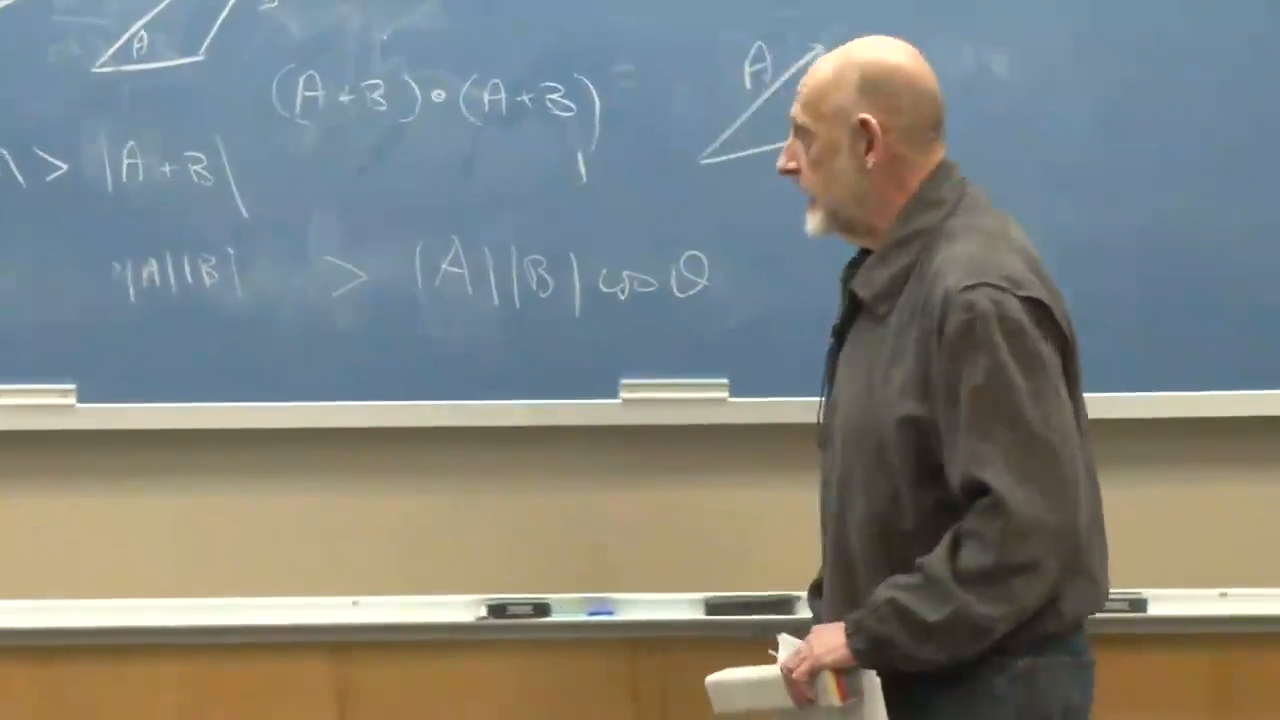
\includegraphics[width=0.88\textwidth]{lecture_10_figure_06.png}
\caption{幾何学的なベクトルの不等式が、証明で用いられるヒルベルト空間のコーシー--シュワルツの限界として書き直される。}
\lectureframe{00:35:35}
\end{figure}

\begin{classroomqa}
\audiencequestion{不等式は厳密であるべきか、それとも等号が成立し得るか。}
\lecturerresponse{それは以上・等しいの関係である。等号は二つのヒルベルト空間ベクトルが線形従属であるときに成立する。この等号条件は後に最小不確定性波束を特定する。}
\end{classroomqa}

両方の変数を中心化し、まず簡略化された黒板での証明をたどる。そこでは\(\psi(x)\)が実数であるとされる。
\begin{equation}
\ket{A}=X\ket{\psi},
\qquad
\ket{B}=P\ket{\psi}.
\label{eq:l10-auxiliary-vectors}
\end{equation}
それらのノルムの二乗はまさに分散である：
\begin{equation}
\braket{A}{A}=(\Delta x)^2,
\qquad
\braket{B}{B}=(\Delta p)^2.
\end{equation}

\begin{figure}[htbp]
\centering
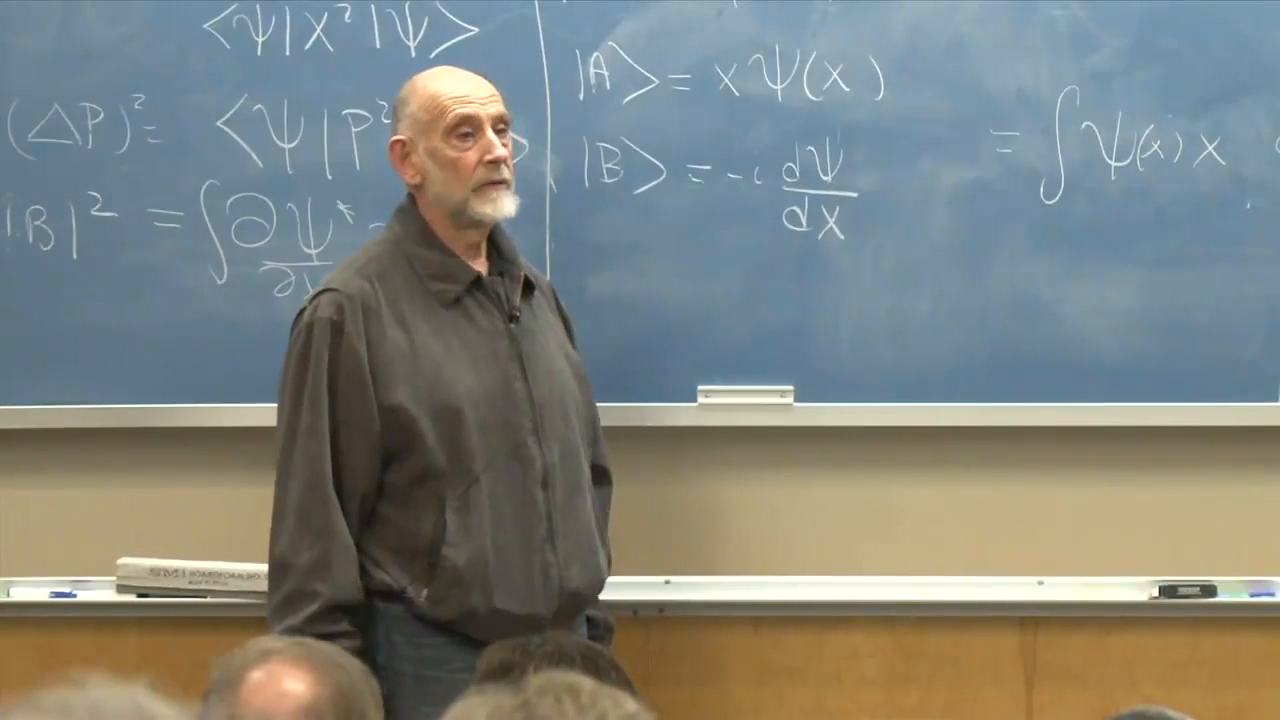
\includegraphics[width=0.88\textwidth]{lecture_10_figure_07.png}
\caption{補助ベクトル\(X\ket{\psi}\)と\(P\ket{\psi}\)が二つの分散をヒルベルト空間のノルムに変える。}
\lectureframe{00:44:40}
\end{figure}

残りの内積は
\begin{align}
\braket{A}{B}
&=
\int_{-\infty}^{\infty}
dx\,
x\psi(x)
\left(-i\hbar\frac{d\psi}{dx}\right).
\end{align}
である。その絶対値のみが寄与する。\(\psi\) は実数であるから、
\begin{equation}
\psi\frac{d\psi}{dx}
=
\frac{1}{2}\frac{d}{dx}\psi^2.
\end{equation}
したがって、
\begin{align}
\left|\braket{A}{B}\right|
&=
\frac{\hbar}{2}
\left|
\int_{-\infty}^{\infty}
dx\,
x\frac{d}{dx}\psi^2
\right| \notag\\
&=
\frac{\hbar}{2}
\left|
-\int_{-\infty}^{\infty}
dx\,\psi^2
\right|
=
\frac{\hbar}{2},
\label{eq:l10-inner-product-half-hbar}
\end{align}
ここで部分積分により \(\psi^2\) から微分が除かれ、\(d x/dx=1\)、境界項は消え、最後の等号は規格化から与えられる。

式~\eqref{eq:l10-inner-product-half-hbar}をCauchy--Schwarzの不等式に代入すると、
\begin{equation}
(\Delta x)^2(\Delta p)^2
\geq
\frac{\hbar^2}{4}.
\end{equation}
正の平方根を取れば、
\begin{equation}
\boxed{
\Delta x\,\Delta p
\geq
\frac{\hbar}{2}
}.
\label{eq:l10-uncertainty-principle}
\end{equation}

\begin{figure}[htbp]
\centering
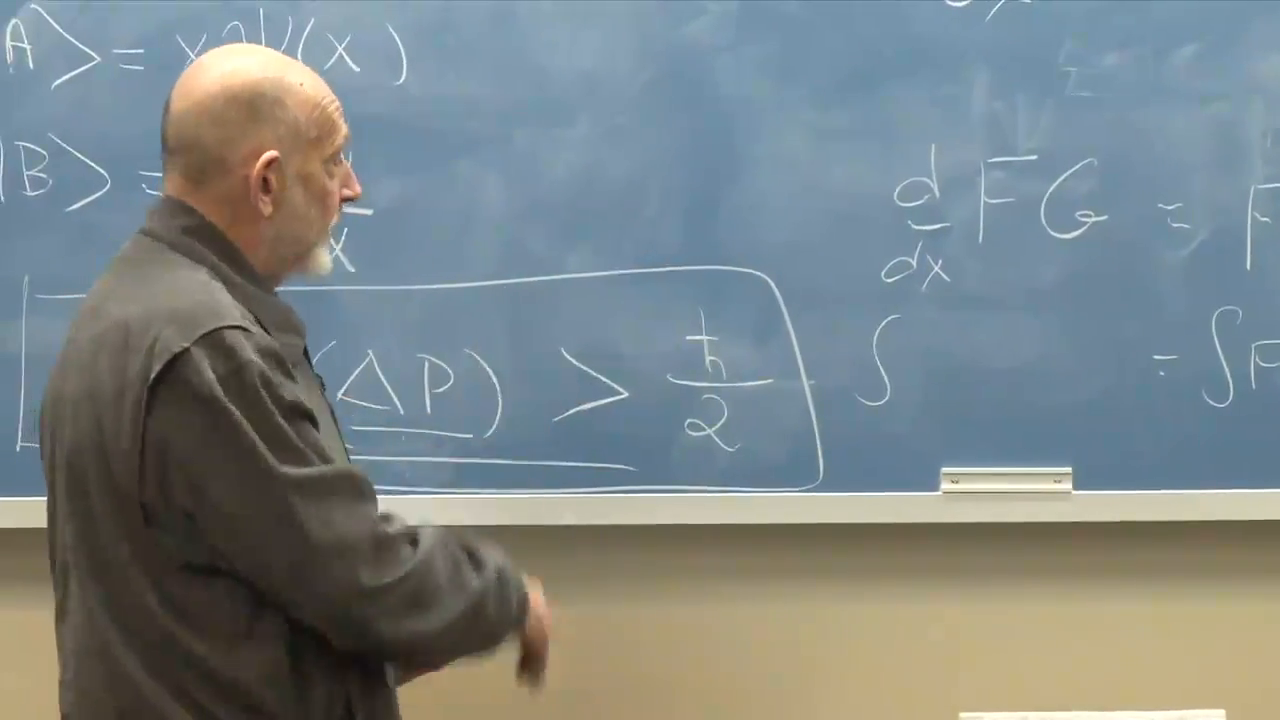
\includegraphics[width=0.88\textwidth]{lecture_10_figure_08.png}
\caption{部分積分の手順と規格化により、位置と運動量の不確定性の鋭い下限が得られる。}
\lectureframe{00:50:55}
\end{figure}

実の \(\psi\) への制限は黒板での便宜上のものであり、定理に対する制限ではなかった。一般の複素状態に対しては、
\begin{equation}
\ket{A}=(X-\expect{X})\ket{\psi},
\qquad
\ket{B}=(P-\expect{P})\ket{\psi}.
\end{equation}
と取る。交換子はそれらの重なりの虚部を定める：
\begin{equation}
\operatorname{Im}\braket{A}{B}
=
\frac{1}{2i}\expect{[X,P]}
=
\frac{\hbar}{2}.
\end{equation}
\(|\braket{A}{B}|\) はその虚部の大きさ以上であるから、同じ下限が従う。

\begin{classroomqa}
\audiencequestion{繰り返しの部分積分において境界項に正確には何が起こったのか。}
\lecturerresponse{ここで考える規格化可能な波束に対しては、\(+\infty\) と \(-\infty\) に現れる積は消える。有限の周期的区間では、端点の項は相殺する。これらの主張が成り立つように演算子の定義域を選ばなければならない；そうでなければ、形式的な操作は正当化されない。}
\end{classroomqa}

\begin{classroomqa}
\audiencequestion{等号は物理的に達成可能なのか、それとも下限は単なる評価にすぎないのか。}
\lecturerresponse{達成可能である。Cauchy--Schwarzの不等式における等号は、二つの補助ベクトルが比例することを要求する。その条件を解くとガウス波束、すなわち次に展開する最小不確定性状態が得られる。}
\end{classroomqa}

\section{他のフーリエ共役対}

時間とエネルギーの不確定性関係は、位置と運動量のそれに似ている。しかし、ここでは時間は通常、普遍的な自己共役演算子で表される観測量ではなく、発展のパラメータであるため、より注意を要する。状態をエネルギー固有ベクトルで展開すると、
\begin{equation}
\ket{\psi(t)}
=
\int dE\,
\phi(E)e^{-iEt/\hbar}\ket{E}.
\label{eq:l10-time-energy-fourier}
\end{equation}
エネルギー振幅と時間的変化はフーリエ関係にある。狭いエネルギー分布はゆっくり変化し、鋭い時間的パルスを作ることはできない；広いエネルギー分布は短い到達時間の包絡線を生み出しうる。

\begin{figure}[htbp]
\centering
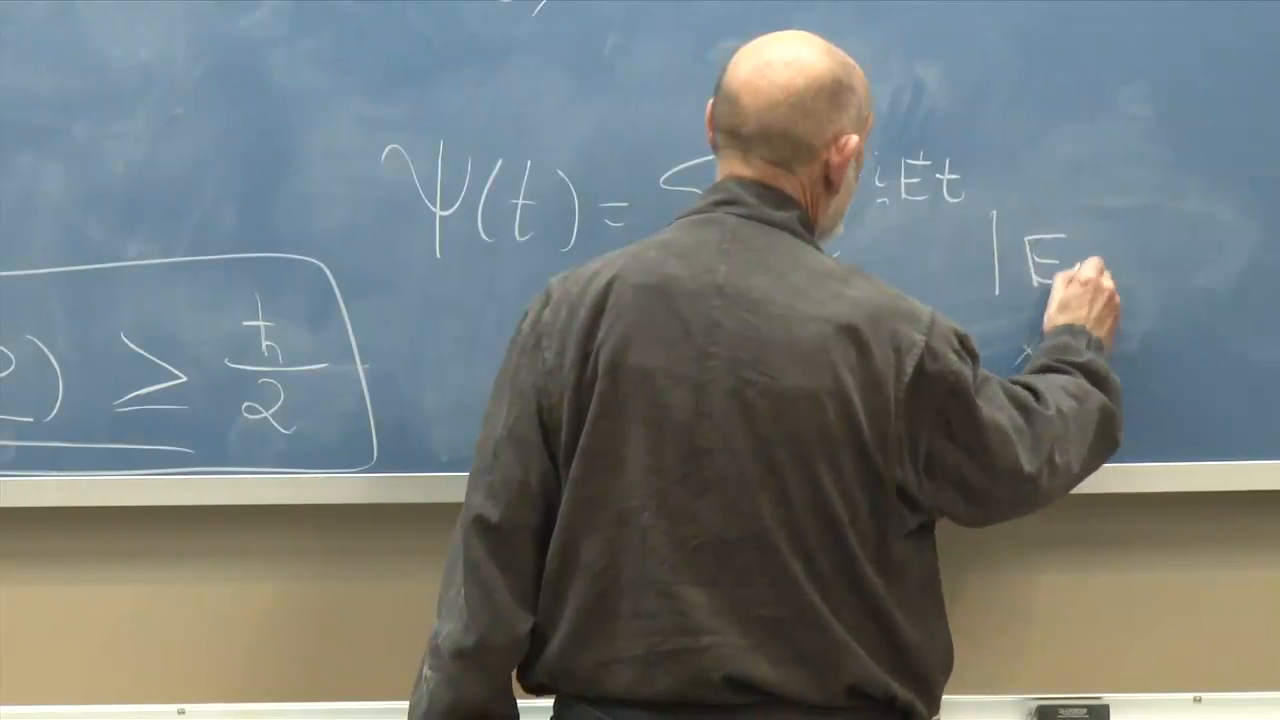
\includegraphics[width=0.88\textwidth]{lecture_10_figure_09.png}
\caption{時間依存性は位相 \(e^{-iEt/\hbar}\) を持つエネルギー固有状態から組み立てられ、時間とエネルギーの関係のフーリエ基底を与える。}
\lectureframe{00:53:40}
\end{figure}

\begin{classroomqa}
\audiencequestion{同じ証明は時間とエネルギーに直接適用できるのか。}
\lecturerresponse{逆幅の直観は適用でき、通過する波束は有用な例を与える：短い到達時間の窓には広いエネルギー分布が必要である。演算子に関する主張はより微妙である。時間はこの定式化において \(X\) と全く同じようには入らないからである。}
\end{classroomqa}

角度と角運動量は回転運動に対するもう一つの共役対をなす。局所的にはそれらのフーリエ関係は位置と運動量に似ている。大域的には角度の周期性がさらなる注意を導入するため、ここでの言及は完全な定理ではなく類推である。

\begin{classroomqa}
\audiencequestion{位置と運動量、時間とエネルギー、角度と角運動量は孤立した例なのか。}
\lecturerresponse{そうではない。正準共役な変数は繰り返しフーリエ対として現れる。定義域と周期性の詳細は異なるが、相互的な局在化が共通の構造である。}
\end{classroomqa}

\section{位置空間におけるSchr\"odinger方程式}

ここで力学に戻る。抽象的な法則は
\begin{equation}
i\hbar\frac{d}{dt}\ket{\psi(t)}
=
H\ket{\psi(t)}.
\label{eq:l10-abstract-schrodinger}
\end{equation}
質量 \(m\) の粒子がポテンシャル \(V(X)\) の中にあるとき、
\begin{equation}
H=\frac{P^2}{2m}+V(X).
\label{eq:l10-particle-hamiltonian}
\end{equation}
と取る。これは古典的な運動エネルギーとポテンシャルの形を取り入れ、その量子発展が適切な領域で古典的運動を再現するかどうかを検証するものである。

\begin{figure}[htbp]
\centering
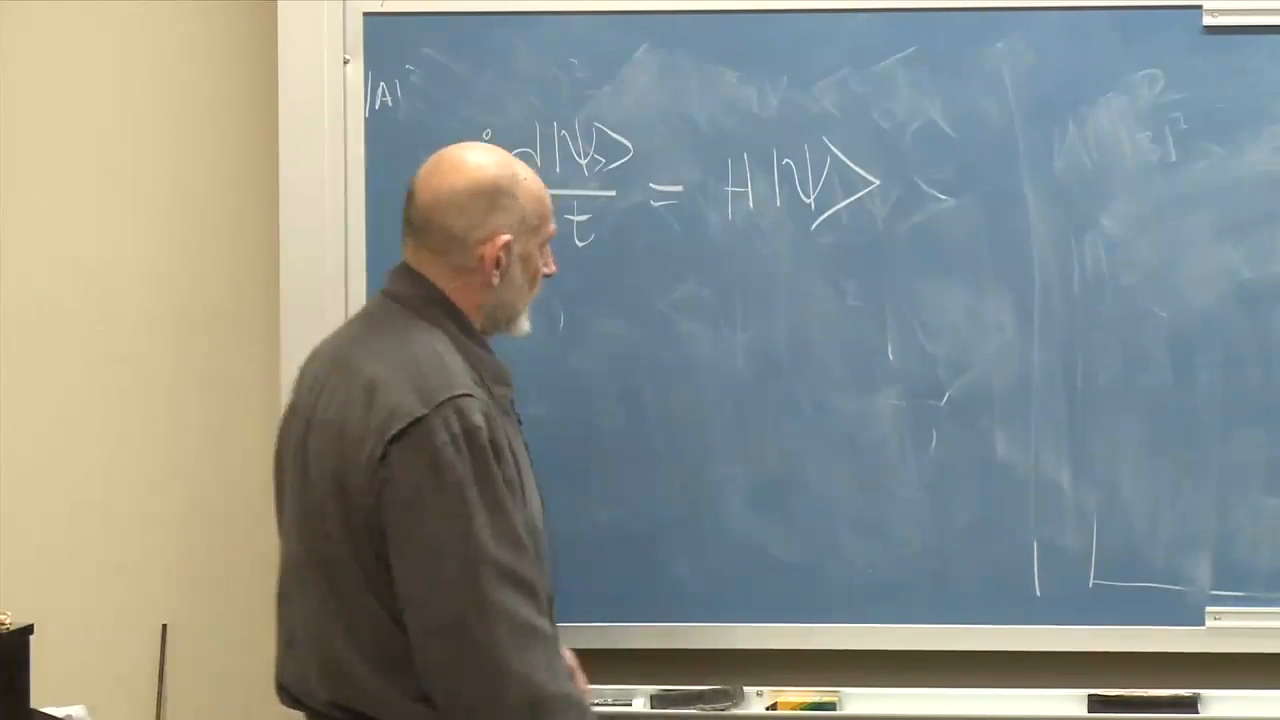
\includegraphics[width=0.88\textwidth]{lecture_10_figure_10.png}
\caption{ハミルトニアンは時間依存Schr\"odinger方程式において抽象状態ベクトルに作用する。}
\lectureframe{00:59:05}
\end{figure}

位置表示では、\(P^2\) は二階微分になる。\(X\) の関数は掛け算として作用する：
\begin{equation}
\bigl(V(X)\psi\bigr)(x)=V(x)\psi(x).
\end{equation}
したがって、
\begin{equation}
i\hbar\frac{\partial\psi(x,t)}{\partial t}
=
\left[
-\frac{\hbar^2}{2m}\frac{\partial^2}{\partial x^2}
+V(x)
\right]\psi(x,t).
\label{eq:l10-position-schrodinger}
\end{equation}

\begin{figure}[htbp]
\centering
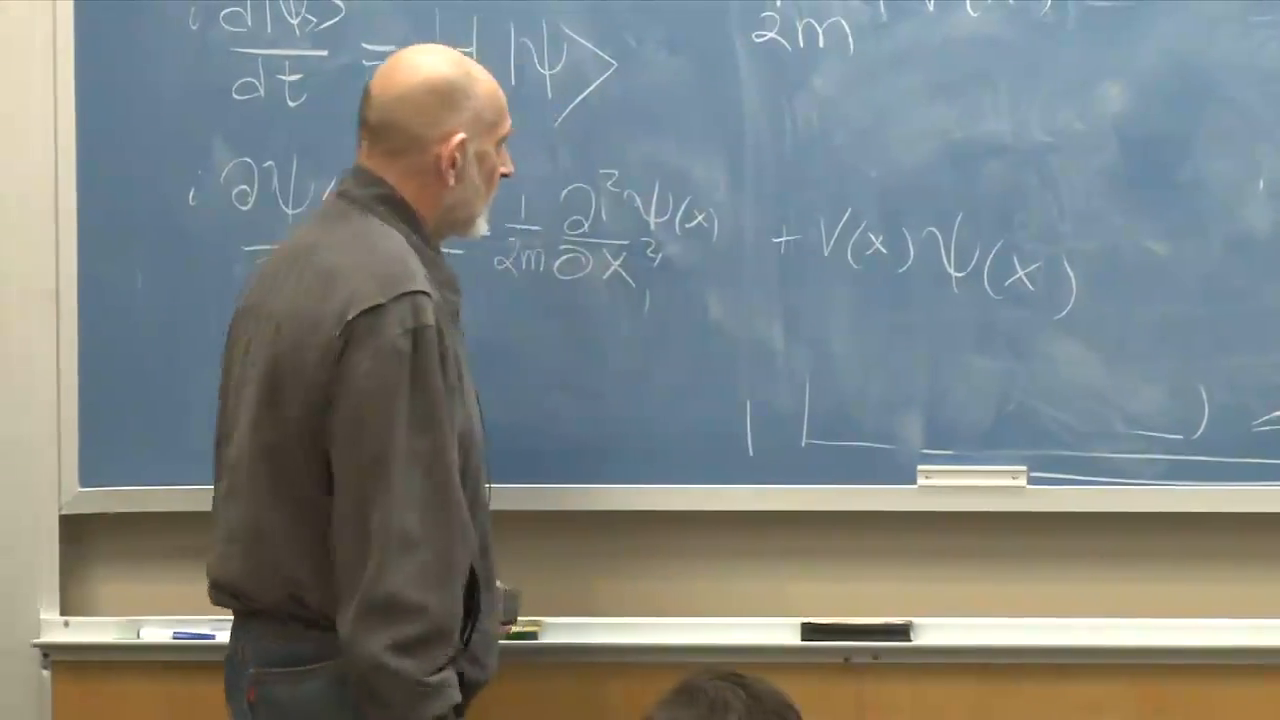
\includegraphics[width=0.88\textwidth]{lecture_10_figure_11.png}
\caption{粒子のハミルトニアンは運動エネルギーの二階微分と \(V(x)\) の掛け算になる。}
\lectureframe{01:03:05}
\end{figure}

\begin{classroomqa}
\audiencequestion{通常の関数 \(V(x)\) はどのような意味で演算子なのか。}
\lecturerresponse{位置基底を選べば、\(X\) は \(x\) を掛けることによって作用する。したがって、十分に正則な関数 \(V(X)\) は各点で対応する数 \(V(x)\) を掛けることによって作用する。その有用性は続く力学によって検証される。}
\end{classroomqa}

期待値の計算のために、式~\eqref{eq:l10-position-schrodinger}を2つの時間微分について解く：
\begin{align}
\dot{\psi}
&=
\frac{i\hbar}{2m}\psi''
-\frac{i}{\hbar}V\psi,
\label{eq:l10-psi-dot}\\
\dot{\psi}^{\,*}
&=
-\frac{i\hbar}{2m}\psi^{*\,\prime\prime}
+\frac{i}{\hbar}V\psi^*.
\label{eq:l10-psi-star-dot}
\end{align}
2行目は1行目の複素共役にすぎないが、両方を書くことで相殺が見えやすくなる。

\section{波束中心の運動}

位置分布の中心は
\begin{equation}
\expect{X}
=
\int_{-\infty}^{\infty}
dx\,\psi^*(x,t)\,x\,\psi(x,t).
\end{equation}
これを微分すると
\begin{equation}
\frac{d}{dt}\expect{X}
=
\int dx\,
\left(
\dot{\psi}^{\,*}x\psi
+
\psi^*x\dot{\psi}
\right).
\label{eq:l10-x-expectation-derivative}
\end{equation}
2つの項は複素共役である。式~\eqref{eq:l10-psi-dot}と\eqref{eq:l10-psi-star-dot}を代入すると、\(V(x)\)は実数であるからポテンシャル項は相殺する。運動項を部分積分すると
\begin{align}
\frac{d}{dt}\expect{X}
&=
\frac{1}{m}
\int dx\,
\psi^*
\left(-i\hbar\frac{\partial}{\partial x}\right)
\psi \notag\\
&=
\frac{\expect{P}}{m}.
\label{eq:l10-ehrenfest-x}
\end{align}

\begin{figure}[htbp]
\centering
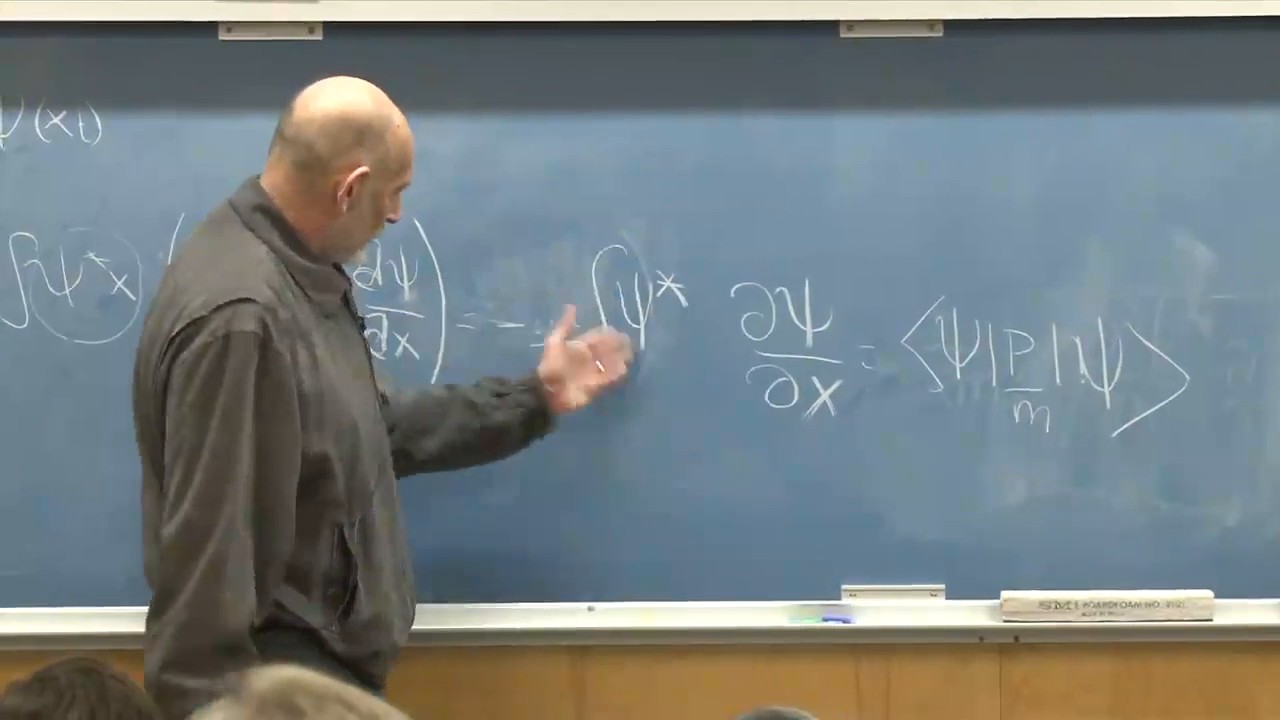
\includegraphics[width=0.88\textwidth]{lecture_10_figure_12.png}
\caption{波束中心の導関数は、運動量の期待値を質量で割ったものに帰着する。}
\lectureframe{01:15:40}
\end{figure}

この関係は厳密である。この代数計算には狭い波束の近似は一切入っていない。

\begin{classroomqa}
\audiencequestion{この導出において、波動関数が単一の狭い山であるという仮定はどこで用いられたのか。}
\lecturerresponse{どこでもない。恒等式\(d\expect{X}/dt=\expect{P}/m\)は、このハミルトニアンの定義域に属するすべての状態に対して成り立つ。局在が問題になるのは、\(\expect{X}\)を古典粒子の軌道と解釈するときだけである。}
\end{classroomqa}

力学のもう半分は運動量に関する：
\begin{equation}
\expect{P}
=
\int dx\,
\psi^*
\left(-i\hbar\frac{\partial}{\partial x}\right)
\psi.
\end{equation}
時間に依存する両方の因子を微分する：
\begin{equation}
\frac{d}{dt}\expect{P}
=
-i\hbar
\int dx\,
\left(
\dot{\psi}^{\,*}\psi'
+
\psi^*\frac{\partial\dot{\psi}}{\partial x}
\right).
\label{eq:l10-p-expectation-start}
\end{equation}
一方の項を部分積分した後、2つのSchr\"odinger方程式を代入する。運動項の寄与は相殺する。ポテンシャル項は次にまとまる：
\begin{equation}
\int dx\,
V(x)
\left(
\psi\frac{\partial\psi^*}{\partial x}
+
\psi^*\frac{\partial\psi}{\partial x}
\right)
=
\int dx\,
V(x)\frac{\partial}{\partial x}|\psi|^2.
\end{equation}
最後にもう一度部分積分して、導関数をポテンシャルに移す：
\begin{align}
\frac{d}{dt}\expect{P}
&=
-\int dx\,|\psi(x,t)|^2\frac{dV}{dx} \notag\\
&=
-\expect{V'(X)}
\\
&=
\expect{F(X)},\\
F(x)&=-V'(x).
\label{eq:l10-ehrenfest-p}
\end{align}

\begin{figure}[htbp]
\centering
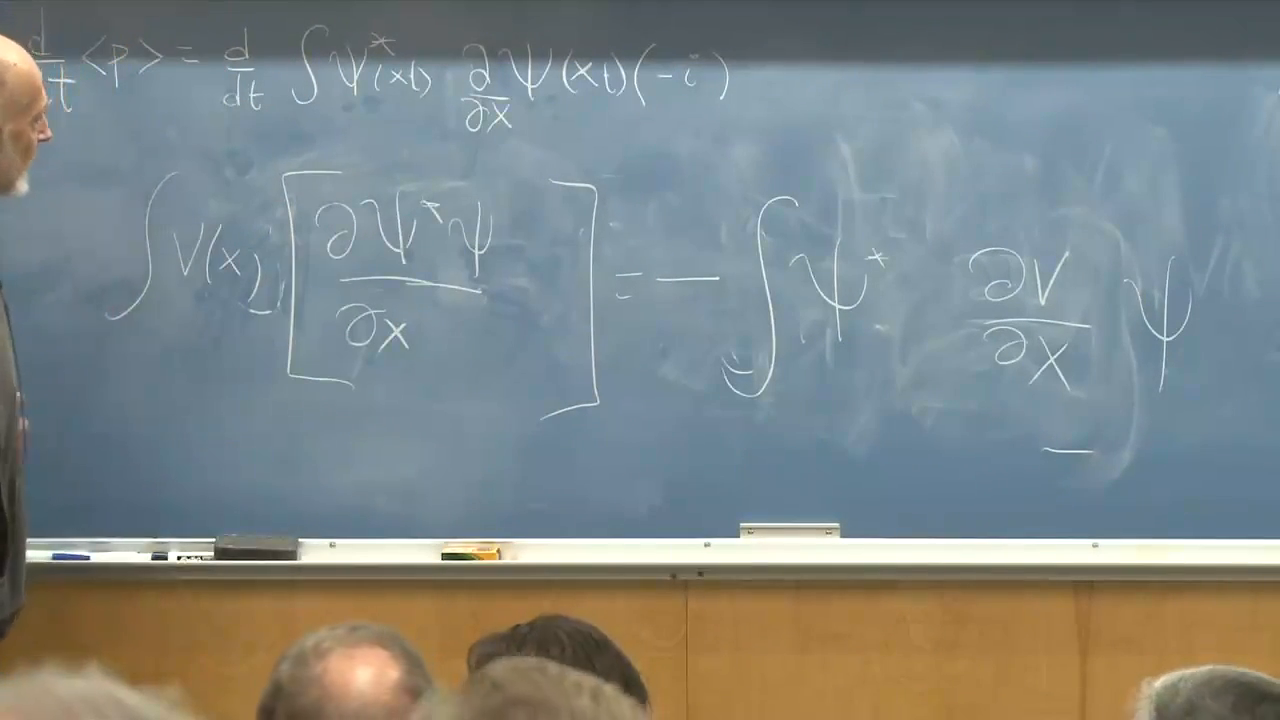
\includegraphics[width=0.88\textwidth]{lecture_10_figure_13.png}
\caption{ポテンシャル項は完全微分にまとまり、\(d\expect{P}/dt=-\expect{V'(X)}\)を与える。}
\lectureframe{01:30:45}
\end{figure}

式~\eqref{eq:l10-ehrenfest-x}と\eqref{eq:l10-ehrenfest-p}は、このハミルトニアンに対するエーレンフェストの定理である。これらは厳密な量子恒等式であるが、厳密な期待値方程式はまだ古典軌道と同じではない。

\section{古典近似はどこで入るか}

波束中心にある点に対する古典力学は次を要求する：
\begin{equation}
\frac{d}{dt}\expect{P}
\approx
F\!\left(\expect{X}\right).
\label{eq:l10-classical-center-force}
\end{equation}
量子力学が与えるのは代わりに
\begin{equation}
\frac{d}{dt}\expect{P}
=
\expect{F(X)}.
\end{equation}
一般には、
\begin{equation}
\expect{F(X)}
\neq
F\!\left(\expect{X}\right).
\label{eq:l10-force-nonlinearity}
\end{equation}

\begin{classroomqa}
\audiencequestion{両方のエーレンフェスト方程式が厳密なら、なぜすべての量子状態がニュートンの法則に従うことをすでに証明していることにならないのか。}
\lecturerresponse{波束中心に対するニュートンの法則は、中心で評価された力を必要とする。厳密な量子方程式には、確率分布全体にわたる力の平均が含まれる。これらはゆっくり変化する力の場の中の狭い波束に対しては一致するが、任意の状態や非線形な力に対しては一致しない。}
\end{classroomqa}

講義の反例はこの区別を紛れもなくする。\(F(x)=x^2\)とし、\(+a\)と\(-a\)の近くを中心とする等しい2つの狭い山を持つ規格化された状態を選ぶ。対称性により
\begin{equation}
\expect{X}=0,
\qquad
F\!\left(\expect{X}\right)=0,
\end{equation}
一方、
\begin{equation}
\expect{F(X)}
=
\expect{X^2}
\approx
a^2>0.
\end{equation}

\begin{figure}[htbp]
\centering
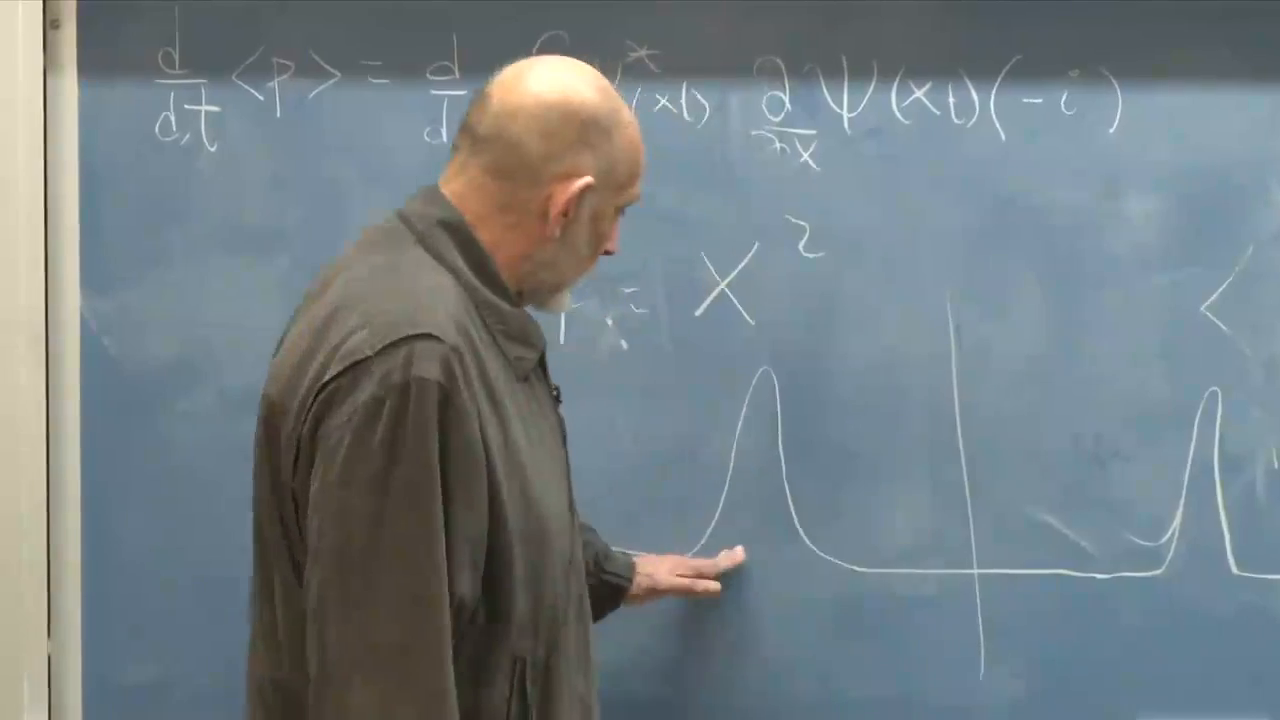
\includegraphics[width=0.88\textwidth]{lecture_10_figure_14.png}
\caption{対称な2つの山を持つ波束と\(F(x)=x^2\)に対して、平均における力は消えるが、力の平均は消えない。}
\lectureframe{01:33:35}
\end{figure}

\(\bar{x}=\expect{X}\)を中心とする単一の狭い波束に対して、力を展開する：
\begin{equation}
F(X)
=
F(\bar{x})
+
F'(\bar{x})(X-\bar{x})
+
\frac{1}{2}F''(\bar{x})(X-\bar{x})^2
+\cdots.
\end{equation}
期待値を取ると線形項は消える：
\begin{equation}
\expect{F(X)}
=
F(\bar{x})
+
\frac{1}{2}F''(\bar{x})(\Delta x)^2
+\cdots.
\end{equation}
古典近似は、力が有意に変化する長さスケールに比べて波束が狭いままでいる場合に信頼できる。

鋭い特徴は波束を分裂させ散乱させうる。広く滑らかなポテンシャルは、十分に局在した波束をその単一の山の形を壊さずに導く傾向がある。点状の障害物、原子核、または波長のスケールの構造は、反射および回折された成分を生じうる。

\begin{figure}[htbp]
\centering
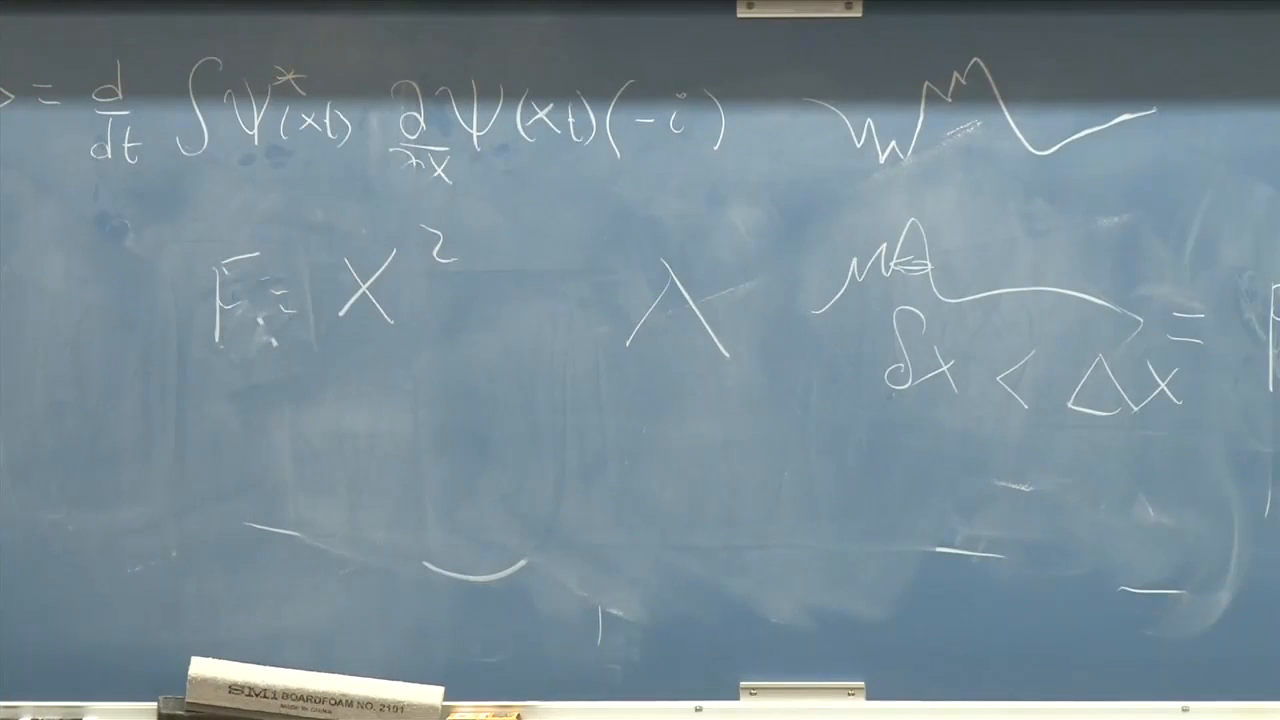
\includegraphics[width=0.88\textwidth]{lecture_10_figure_15.png}
\caption{波束の幅または関連する波長より短いスケールのポテンシャル構造は、コヒーレントな波束を散乱成分に分解しうる。}
\lectureframe{01:37:25}
\end{figure}

\begin{classroomqa}
\audiencequestion{ポテンシャルが古典的な波束にとって悪いものになるのはなぜか。}
\lecturerresponse{問題はスケールであり、道徳的な性質ではない。波束よりはるかに鋭い特徴、またはその波長と同程度の特徴は、波動としての性質を顕在化させ、散乱を生じる。ポテンシャルが波束にわたってゆっくり変化するなら、力はその台の上でほぼ一定であり、中心は古典方程式に従う。}
\end{classroomqa}

質量も重要である。ほぼ最小不確定性の波束に対して、
\begin{equation}
\Delta x\,\Delta v
\sim
\frac{\hbar}{2m}.
\end{equation}
大きな質量は、小さな空間的幅と適度な速度の広がりの両方を可能にする。したがって重い物体は、巨視的なポテンシャルを通過する間も鋭く局在したままでいられる。軽い粒子は、微視的構造によってより容易に広げられたり回折されたりする。これはスケーリングの議論であり、質量だけが運動が古典的かどうかを決めるという主張ではない。

\begin{classroomqa}
\audiencequestion{この意味で、電子が近似的に古典的に振る舞うほど大きくなることはあるのだろうか。}
\lecturerresponse{ある。外部場が電子の波束の尺度で滑らかに変化するならば。例えば広いコンデンサー板の間では、コヒーレントな波束は有用な時間にわたって古典的な加速度に従うことができる。原子核の鋭いクーロン構造の近くでは、同じ電子が顕著な散乱を示す。}
\end{classroomqa}

ラザフォードの1911年の散乱実験は補完的な教訓を与える。金原子核のコンパクトな電荷分布に出会ったアルファ粒子は大きな角度で散乱され、正電荷が非常に小さな領域に集中していることが明らかになった。ラザフォードは粒子のビームを記述し、量子力学は入射振幅とその散乱成分を記述する。現代の電子および光子の散乱実験も同じ尺度感度を利用している。

\begin{classroomqa}
\audiencequestion{この波対尺度の振る舞いは物質粒子に特有のものだろうか。}
\lecturerresponse{いいえ。電磁波は、屈折率が一つの波長にわたってゆっくり変化するとき、幾何光学に従う。波長と同程度の間隔をもつ回折格子は、波を異なる方向へ広げる。電子、アルファ粒子、光子、その他の量子励起は、波長と構造の間のこの関係を共有している。}
\end{classroomqa}

したがって古典極限は、量子力学に貼り付けられた別個の法則ではない。厳密な期待値方程式はすでに古典的関係を含んでいる。古典的軌道は、状態が局在したままであり、ハミルトニアンが十分滑らかに変化して、力を平均することが事実上波束中心でそれを評価することと同じになる場合に現れる。
